\documentclass[conference]{IEEEtran}

\usepackage[utf8]{inputenc}
\usepackage[T1]{fontenc}
\usepackage{cite}
\usepackage{url}
\usepackage{graphicx}
\usepackage{booktabs}
\usepackage{array}
\usepackage{amsmath}
\usepackage{microtype}

\graphicspath{{../figures/}}

\title{Breaking the Windows Compatibility Barrier:\\
Engineering Linux Adoption through SteamOS, Bazzite, and Proton}

\author{
\IEEEauthorblockN{Ruggio}
\IEEEauthorblockA{
RT2 Assignment 2\\
University of Genoa\\
}
}

\begin{document}

\maketitle

\begin{abstract}
Desktop Linux adoption is often discussed as a problem of usability, hardware support or user preference. This paper instead focuses on the application-ecosystem barrier between Windows and Linux. Even when Linux is technically suitable, users and organisations may remain dependent on Windows because required applications rely on Windows-specific APIs, drivers, licensing systems, services, file formats or workflows.

The paper presents a state-of-the-art analysis of Windows application compatibility on Linux, with Wine as the general compatibility-layer foundation, Proton and SteamOS as the main technical case study, and Bazzite as a comparative SteamOS-like Linux distribution. Proton is analysed as an example of how compatibility-layer engineering can support complex Windows workloads through API translation, graphics translation, runtime management and platform integration. Bazzite is used to discuss the distribution-level side of adoption: preconfiguration, update safety, rollback, packaging and reduced setup friction.

A synthetic experiment is then introduced to operationalise the compatibility-barrier taxonomy. The experiment models how different dependency classes affect simulated compatibility outcomes under five strategies: native Linux, Wine-like compatibility, Proton-like compatibility, managed prefixes and virtualisation. The results are not real-world compatibility measurements. They are used as a structured illustration of why dependency type matters more than nominal application class.

The analysis suggests that compatibility layers can reduce the Windows--Linux application barrier for many user-space workloads, but cannot independently eliminate ecosystem lock-in. Kernel drivers, anti-cheat systems, proprietary licensing, specialised hardware, cloud services and enterprise workflows remain difficult barriers. Linux adoption therefore depends on both compatibility-layer engineering and broader ecosystem integration.
\end{abstract}

\begin{IEEEkeywords}
Linux adoption, Windows compatibility, Wine, Proton, SteamOS, Bazzite, compatibility layers, application portability, vendor lock-in, interoperability.
\end{IEEEkeywords}

\section{Introduction}

Desktop operating systems are not adopted in isolation. A user does not choose only a kernel, graphical shell or package manager; they choose an application ecosystem. For this reason, the migration from Windows to Linux is constrained not only by Linux's technical capabilities, but also by the availability and reliability of required applications.

This issue is visible in many contexts. A home user may depend on a Windows-only game launcher, a professional may require specialised creative or CAD software, and an organisation may rely on internal applications, macros, file formats or peripherals designed around Windows. In each case, the operating-system choice is shaped by the application layer.

The central problem of this paper is therefore the Windows--Linux application compatibility barrier. This barrier is not a single technical defect. It is a set of interacting dependencies involving APIs, graphics stacks, drivers, licensing mechanisms, hardware, cloud services and workflows.

Compatibility layers attempt to reduce this barrier by allowing Windows binaries to run on Linux without a complete rewrite. Wine is the general-purpose compatibility-layer foundation for running Windows applications on POSIX-compliant systems such as Linux, macOS and BSD \cite{winehqAbout}. Proton is a Valve-maintained compatibility tool for Steam Play, based on Wine and additional components, that allows many Windows games to run on Linux through the Steam client \cite{valveProton}. SteamOS provides a Linux-based platform where this compatibility stack can be integrated into a user-facing system \cite{steamOSDownload}. Bazzite is relevant as a comparative distribution-level case because it shows how a SteamOS-like Linux experience can be assembled with gaming-focused preconfiguration and atomic desktop practices \cite{bazziteDocs,bazziteFedoraAtomicComparison}.

The paper does not argue that compatibility layers make Windows irrelevant. Instead, it asks a narrower question: to what extent can compatibility-layer engineering reduce application-related switching costs, and which dependencies continue to block reliable migration?

\subsection{Research Question}

The main research question is:

\begin{quote}
To what extent can compatibility layers reduce the application-ecosystem barrier between Windows and Linux, and which technical dependencies still prevent Windows applications from running reliably without native porting?
\end{quote}

\subsection{Contribution}

The contribution of the paper is fourfold:
\begin{enumerate}
    \item it organises the state of the art around Wine, Proton, SteamOS, Bazzite and related compatibility tools;
    \item it proposes a taxonomy of Windows--Linux compatibility barriers;
    \item it distinguishes technical compatibility from distribution-level adoption friction;
    \item it introduces a synthetic experiment that models how dependency types affect simulated compatibility outcomes.
\end{enumerate}

\subsection{Scope}

The project is not only about videogames. Games are used because they are demanding Windows workloads: they may require Direct3D, launchers, DRM, anti-cheat, input handling, audio, networking and performance-sensitive execution. The success of Proton is therefore technically significant.

However, the broader topic is Windows application portability. The paper also considers productivity, creative, CAD/engineering, scientific and enterprise legacy software as categories where Windows dependence may appear in different forms.

\section{Background and State of the Art}

\subsection{Native Porting, Compatibility Layers, Virtualisation and Emulation}

There are several ways to make a Windows application available to Linux users.

A native Linux port adapts or rebuilds the application so that it runs directly on Linux. This is usually the cleanest solution from the user's perspective, but it requires vendor commitment and long-term maintenance.

A compatibility layer allows a Windows binary to run by recreating or translating the Windows runtime environment expected by the application. Wine belongs to this category. Wine explicitly describes itself as a compatibility layer rather than as a full emulator \cite{winehqAbout}. Recent research also studies OS compatibility layers as a development target in their own right, rather than as marginal legacy tools \cite{lefeuvre2023loupe}.

Virtualisation runs a complete Windows guest operating system inside a virtual machine. It can provide broader compatibility for difficult software, but it retains a strong dependency on Windows licensing, Windows updates and a separated guest environment.

Emulation reproduces hardware or platform behaviour at a lower level. It is not the main focus of this paper. Wine and Proton should not be described as full-system emulators.

The distinction matters because each strategy solves a different part of the compatibility problem. Native porting removes Windows dependency but requires developer effort. Compatibility layers reduce dependency without requiring a port, but remain incomplete. Virtualisation preserves compatibility but does not remove Windows dependence.

\subsection{Wine as the General Compatibility Foundation}

Wine is the foundational project for running Windows applications on Linux and other POSIX-compliant systems. Its importance lies in the fact that it does not require a full copy of Windows. Instead, it implements or translates the interfaces expected by Windows applications \cite{winehqAbout}.

For the Windows--Linux migration problem, Wine is important because it targets existing Windows binaries. It therefore addresses the legacy software problem: applications that already exist for Windows but have no native Linux version.

However, Wine also reveals the limits of compatibility-layer approaches. Applications may rely on undocumented behaviour, missing APIs, Windows services, drivers, licensing systems or hardware assumptions. In these cases, compatibility is not guaranteed by the presence of the compatibility layer alone. There are also security implications when running Windows software and potentially Windows malware through Wine on Linux systems \cite{duncan2019wineSecurity}.

Wine should therefore be treated as a general-purpose foundation rather than a universal solution.

\subsection{Proton as a Specialised Wine-Based Compatibility Stack}

Proton is built for the Steam ecosystem. Valve describes Proton as a tool used with the Steam client that allows Windows-exclusive games to run on Linux \cite{valveProton}. It is based on Wine and additional components, and its technical importance comes from integration rather than from a single mechanism.

Proton combines several layers:
\begin{itemize}
    \item Wine-based Windows API compatibility;
    \item graphics translation through components such as DXVK and VKD3D-Proton;
    \item Steam integration;
    \item runtime and dependency control;
    \item game-specific fixes and compatibility configuration.
\end{itemize}

DXVK provides a Vulkan-based implementation of Direct3D 8, 9, 10 and 11 for Linux/Wine \cite{dxvk}. VKD3D-Proton targets Direct3D 12 translation on top of Vulkan for Proton \cite{vkd3dProton}. Steam Runtime is relevant because it helps control dependencies and execution environments for Steam applications \cite{steamRuntime}.

This makes Proton a strong case study because modern Windows games are complex. If a compatibility stack can support many game workloads, then compatibility-layer engineering is not limited to simple legacy applications.

Nevertheless, Proton's domain matters. It is optimised for Steam and gaming. It should not be used as proof that all Windows applications can run on Linux. Enterprise software, CAD tools, professional licensing systems, hardware dongles and specialised drivers introduce different constraints.

\subsection{SteamOS as Platform Integration}

SteamOS is important because it shows that compatibility is not only a library-level problem. A compatibility layer must be integrated into a usable system. From the user's perspective, it matters whether games or applications are easy to launch, whether updates break existing setups, whether the runtime is stable and whether hardware behaves consistently.

This platform layer can also involve display and session-management components, such as gamescope, which illustrates that compatibility is affected by the surrounding desktop and runtime environment as well as by Wine or Proton themselves \cite{gamescope}.

SteamOS and Steam Deck also introduce user-facing compatibility classification through the Steam Deck compatibility review process \cite{steamDeckCompatibility}. This is relevant because compatibility is not binary. An application may be fully supported, partially usable, require manual configuration, or fail due to specific dependencies.

The SteamOS/Proton case therefore suggests that compatibility-layer adoption requires:
\begin{itemize}
    \item technical translation;
    \item runtime stability;
    \item platform integration;
    \item compatibility metadata;
    \item user-facing expectations;
    \item update management.
\end{itemize}

\subsection{Bazzite as a Distribution-Level Adoption Case}

Bazzite is useful in this paper not because it is the same as SteamOS, but because it provides a comparative SteamOS-like Linux distribution case. Its documentation compares it with Fedora Atomic Desktop and highlights gaming-focused preinstalled software such as Steam and Lutris, together with Distrobox containers for accessing other Linux package-management environments \cite{bazziteFedoraAtomicComparison,bazziteGamingIntro}. Fedora Atomic Desktops provide the broader atomic desktop context behind this distribution-level model \cite{fedoraAtomicDesktops}.

This is relevant for the adoption side of the compatibility problem. A compatibility layer may exist, but users still need a distribution environment where drivers, launchers, runtimes and updates are manageable. Bazzite represents this distribution-level layer.

The role of Bazzite in the paper is therefore limited and specific: Bazzite does not directly solve Windows API compatibility. It can reduce adoption friction around setup, packaging, updates and usability.

This distinction prevents the paper from confusing compatibility engineering with distribution engineering.

\subsection{Related Compatibility Tools}

Other tools such as Bottles, CrossOver, Lutris and Heroic show that the compatibility ecosystem extends beyond Wine and Proton alone. Their relevance lies in prefix management, dependency management, launcher integration and user experience \cite{bottlesDocs,codeweaversCrossover,lutris,heroicGamesLauncher}.

These tools support the broader argument that Windows compatibility on Linux is not simply a yes/no property. It is mediated by configuration, application profiles, runtime versions, launchers, installers and user-facing workflows.

\subsection{Lock-in and Interoperability}

The compatibility problem also has an economic and organisational dimension. Users may be locked into Windows not because they prefer Windows itself, but because their applications, documents, services and workflows depend on it.

Compatibility layers can reduce some switching costs by allowing selected Windows applications to run on Linux. However, they cannot fully eliminate lock-in where the dependency is contractual, organisational, cloud-based, hardware-bound or tied to proprietary services.

This paper therefore treats compatibility as a socio-technical issue. Technical API translation is necessary but not sufficient for migration. The open-source policy context is relevant as background because open technologies can support interoperability and reduce single-vendor dependency, although this paper does not perform a full policy analysis \cite{ecOpenSourceStrategy2020,euOpenSourceStrategy2026}.

\section{Compatibility Barrier Taxonomy}

The paper classifies compatibility barriers into seven categories.

\subsection{User-Space API Dependency}

Applications may depend on Windows-specific APIs, libraries or runtime behaviour. Examples include Win32, COM, .NET Framework, registry assumptions, drive-letter paths and Windows-specific file-system behaviour. These dependencies are the traditional target of Wine-like compatibility layers.

\subsection{Graphics Stack Dependency}

Graphics-heavy applications may depend on Direct3D or specific GPU assumptions. Proton's technical success is closely connected to graphics translation from Direct3D to Vulkan through projects such as DXVK and VKD3D-Proton \cite{dxvk,vkd3dProton}. This category is especially important for games, creative tools and some CAD/engineering applications.

\subsection{Kernel and Driver Dependency}

Some applications require privileged services or kernel-level components. These are more difficult for compatibility layers because they depend on low-level Windows behaviour rather than user-space APIs.

Examples include anti-cheat drivers, VPN drivers, kernel-level DRM, hardware protection dongles and specialised device drivers. Kernel-level anti-cheat systems are especially relevant because they interact with operating-system security boundaries and can create compatibility and trust problems \cite{dorner2024anticheat,areWeAntiCheatYet}.

\subsection{Licensing and DRM Dependency}

An application may technically start under a compatibility layer but fail because its licensing system expects Windows-specific hardware identifiers, online activation behaviour, kernel services or vendor-controlled cloud services. This is a major barrier for professional and enterprise software.

\subsection{Hardware Dependency}

Scientific, industrial, medical, audio, creative and engineering tools may depend on specialised peripherals. If the required hardware has no Linux driver or expects a Windows-only driver stack, compatibility layers cannot fully solve the problem.

\subsection{Workflow Dependency}

A workflow may depend on more than the application binary. It may involve macros, file formats, templates, plugins, network drives, internal scripts, authentication systems or collaborative platforms. This category is important because migration failure can occur even when the main application technically runs.

\subsection{Distribution-Level Friction}

Finally, users may face friction from setup complexity, unstable updates, driver configuration, runtime conflicts and lack of documentation. This is why SteamOS and Bazzite are relevant: they address the environment around compatibility rather than only the compatibility layer itself.

\section{Methodology}

\subsection{Literature Review}

The literature review is organised through the repository material: the search protocol, the source matrix and the source notes. The review combines official documentation, maintainer repositories, academic papers and supporting community sources. These sources are grouped thematically instead of being summarised one by one.

The evidence hierarchy is:
\begin{enumerate}
    \item peer-reviewed research;
    \item official technical documentation;
    \item maintainer repositories;
    \item community compatibility databases;
    \item blogs and opinion pieces only for context.
\end{enumerate}

\subsection{Synthetic Experiment}

The experimental design is documented in the repository, while the Jupyter notebook contains the executable synthetic model used to generate the dataset, processed results and figures.

The experiment is synthetic. Its role is to make the taxonomy operational by simulating how different dependency classes affect compatibility outcomes. The model compares five strategies: native Linux, Wine-like execution, Proton-like compatibility, managed prefixes and virtualisation.

The model includes six application classes: productivity, creative, CAD/engineering, scientific, enterprise legacy and games. The dataset contains $6$ application classes, $5$ strategies and $20$ trials for each class-strategy combination, for a total of $600$ rows.

\subsection{Variables}

The independent variables are application class, compatibility strategy, API dependency level, kernel dependency level, hardware dependency level, licensing dependency level and packaging support.

The dependent variables are compatibility outcome, compatibility score, setup effort, runtime overhead, integration score and retained Windows dependency.

\subsection{Interpretation Rule}

The experiment is not used as empirical proof. It is used as a controlled model. Results should be read as ``given these assumptions, this is how dependency classes interact'', not as ``this is the real compatibility rate of Linux, Wine, Proton or Bazzite''.

\section{Experimental Results}

\subsection{Dataset Overview}

The experiment produces a raw synthetic dataset and a processed strategy-level summary. The dataset contains 600 rows, and each strategy is evaluated through 120 synthetic trials.

\subsection{Aggregated Results by Strategy}

Table~\ref{tab:aggregated-results} reports the strategy-level results.

\begin{table*}[t]
\centering
\caption{Aggregated synthetic results by compatibility strategy. Values are model outputs, not real-world benchmark measurements.}
\label{tab:aggregated-results}
\begin{tabular}{lrrrrrrr}
\toprule
Strategy & Trials & Mean score & Setup effort & Runtime overhead & Integration & Windows retained & Full rate \\
\midrule
native\_linux   & 120 & 89.086 & 11.170 &  3.803 & 95.695 & 0.000 & 0.992 \\
virtualisation & 120 & 80.110 & 49.925 & 25.956 & 46.403 & 1.000 & 0.742 \\
proton\_like   & 120 & 49.910 & 41.915 &  9.627 & 79.698 & 0.000 & 0.050 \\
managed\_prefix & 120 & 45.462 & 34.660 & 11.881 & 75.366 & 0.000 & 0.033 \\
wine\_like     & 120 & 24.776 & 81.800 & 13.860 & 60.850 & 0.000 & 0.000 \\
\bottomrule
\end{tabular}
\end{table*}

These values are synthetic. They reflect the assumptions encoded in the model, not observed real-world compatibility rates.

\subsection{Interpretation}

The synthetic results follow the intended logic of the model. Native Linux is the strongest strategy when available. It has the highest mean compatibility score, the lowest setup effort and the highest integration score. This reflects the fact that native applications avoid most Windows compatibility translation problems.

Virtualisation has a high compatibility score, but it retains a complete Windows dependency. It also has higher runtime overhead and lower Linux integration. This supports the distinction between compatibility and actual migration away from Windows.

The Proton-like strategy performs better than raw Wine-like execution in integration and runtime overhead, but its full compatibility rate remains low across the full synthetic dataset. This result should not be interpreted as a negative claim about Proton. It reflects the model's inclusion of non-gaming application classes such as CAD, scientific and enterprise software, where Proton-like assumptions are less directly applicable.

Managed prefixes reduce setup effort compared with raw Wine-like execution. This supports the claim that tooling and configuration management matter. However, managed prefixes do not eliminate barriers such as kernel drivers, licensing systems or proprietary hardware dependencies.

Raw Wine-like execution is the most fragile strategy in the model. This reflects high setup sensitivity and the absence of application-specific profiles or platform integration.

\subsection{Figures}

Three figures are included to summarise the synthetic experiment: a strategy comparison, a dependency-risk heatmap and a setup-effort distribution.

\begin{figure}[t]
    \centering
    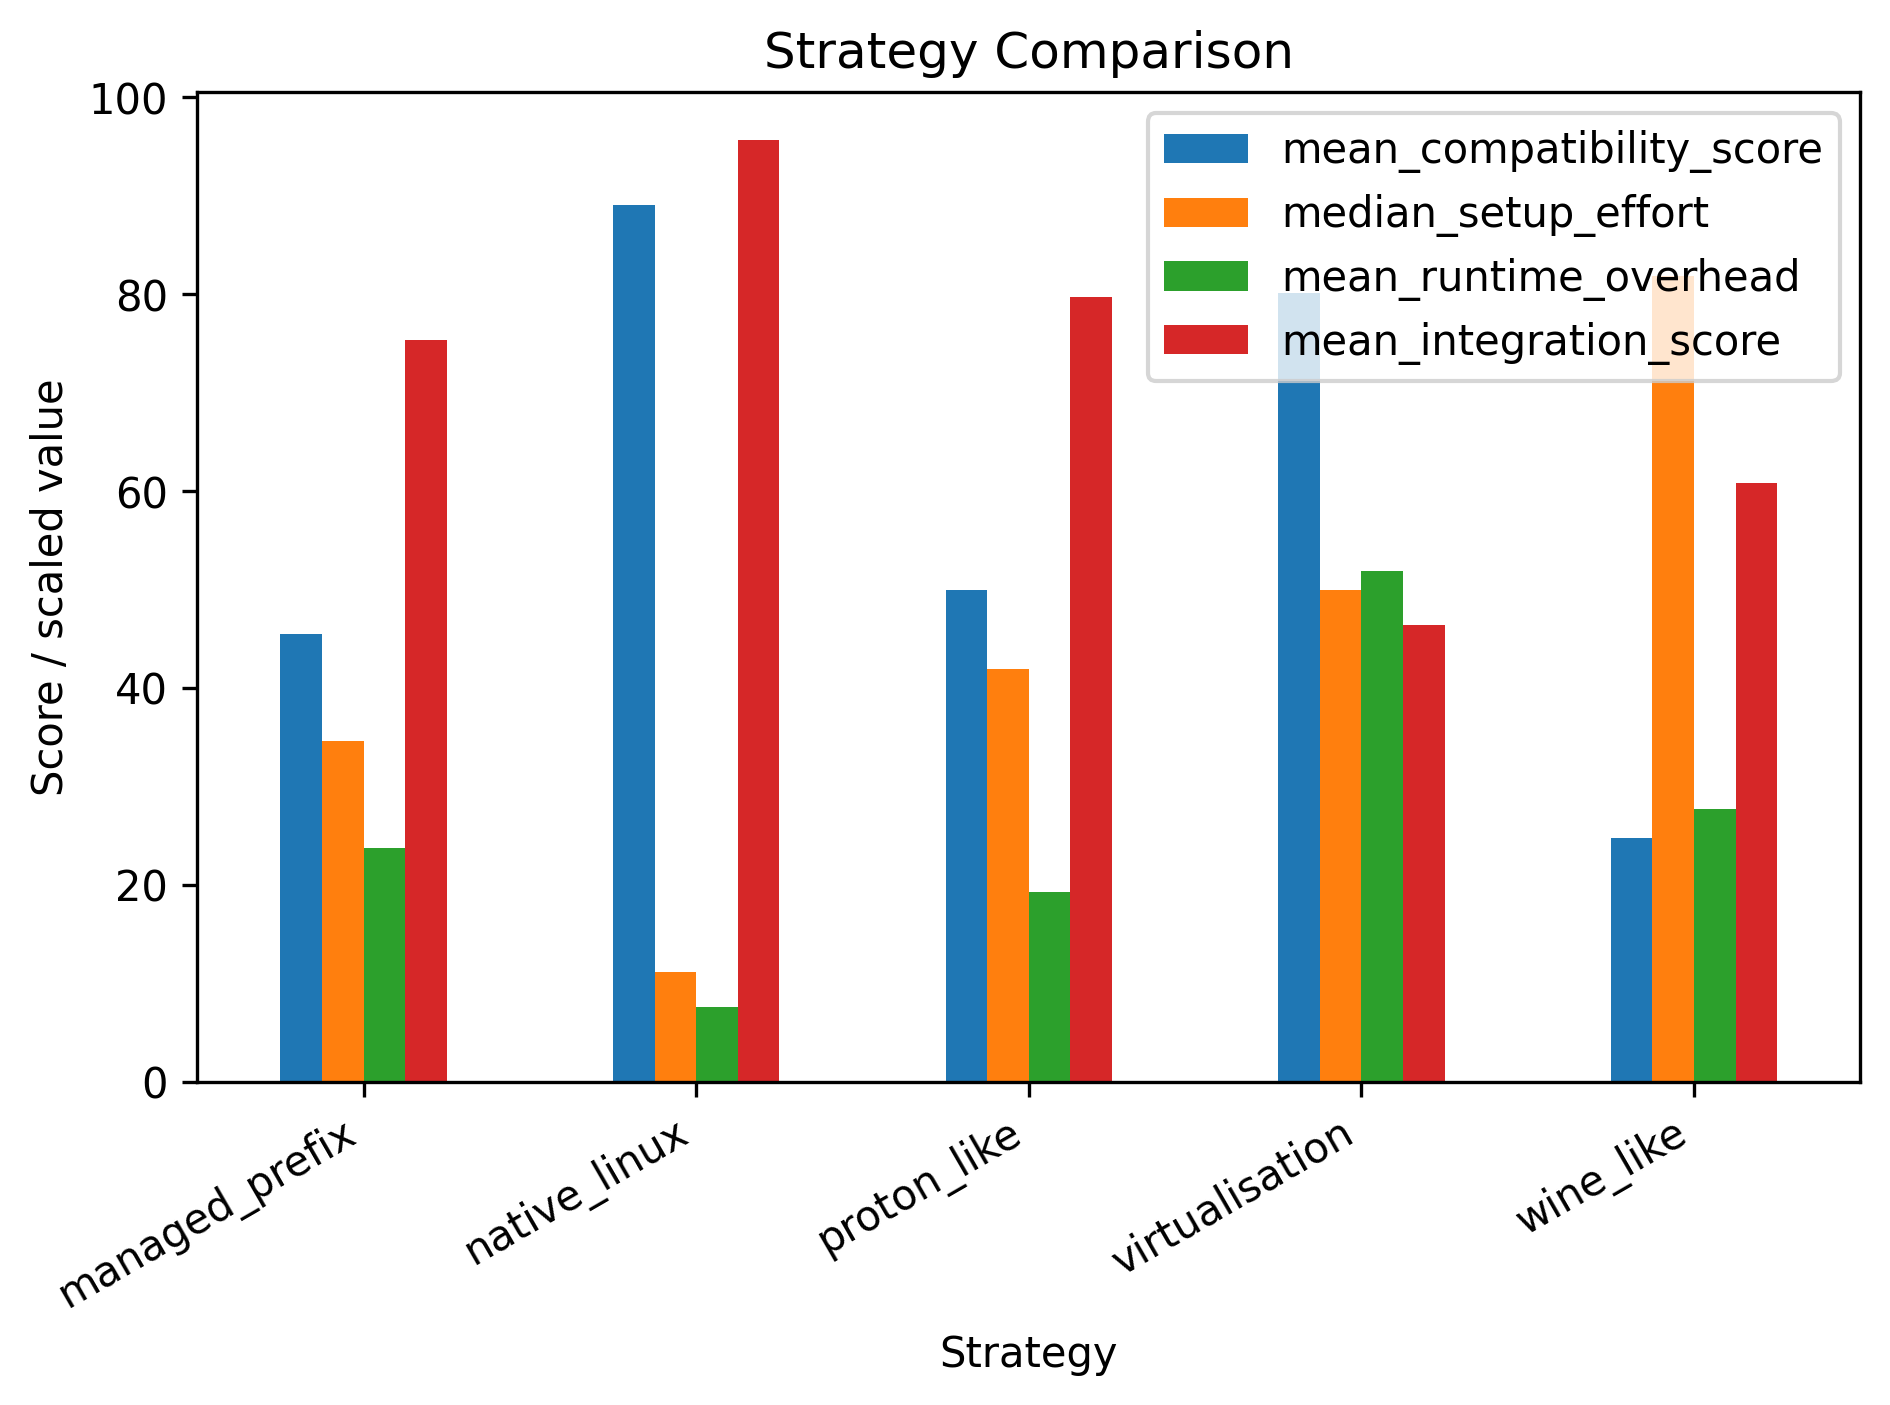
\includegraphics[width=\linewidth]{strategy_comparison.png}
    \caption{Synthetic strategy comparison across compatibility score, setup effort, runtime overhead and integration score.}
    \label{fig:strategy-comparison}
\end{figure}

\begin{figure}[t]
    \centering
    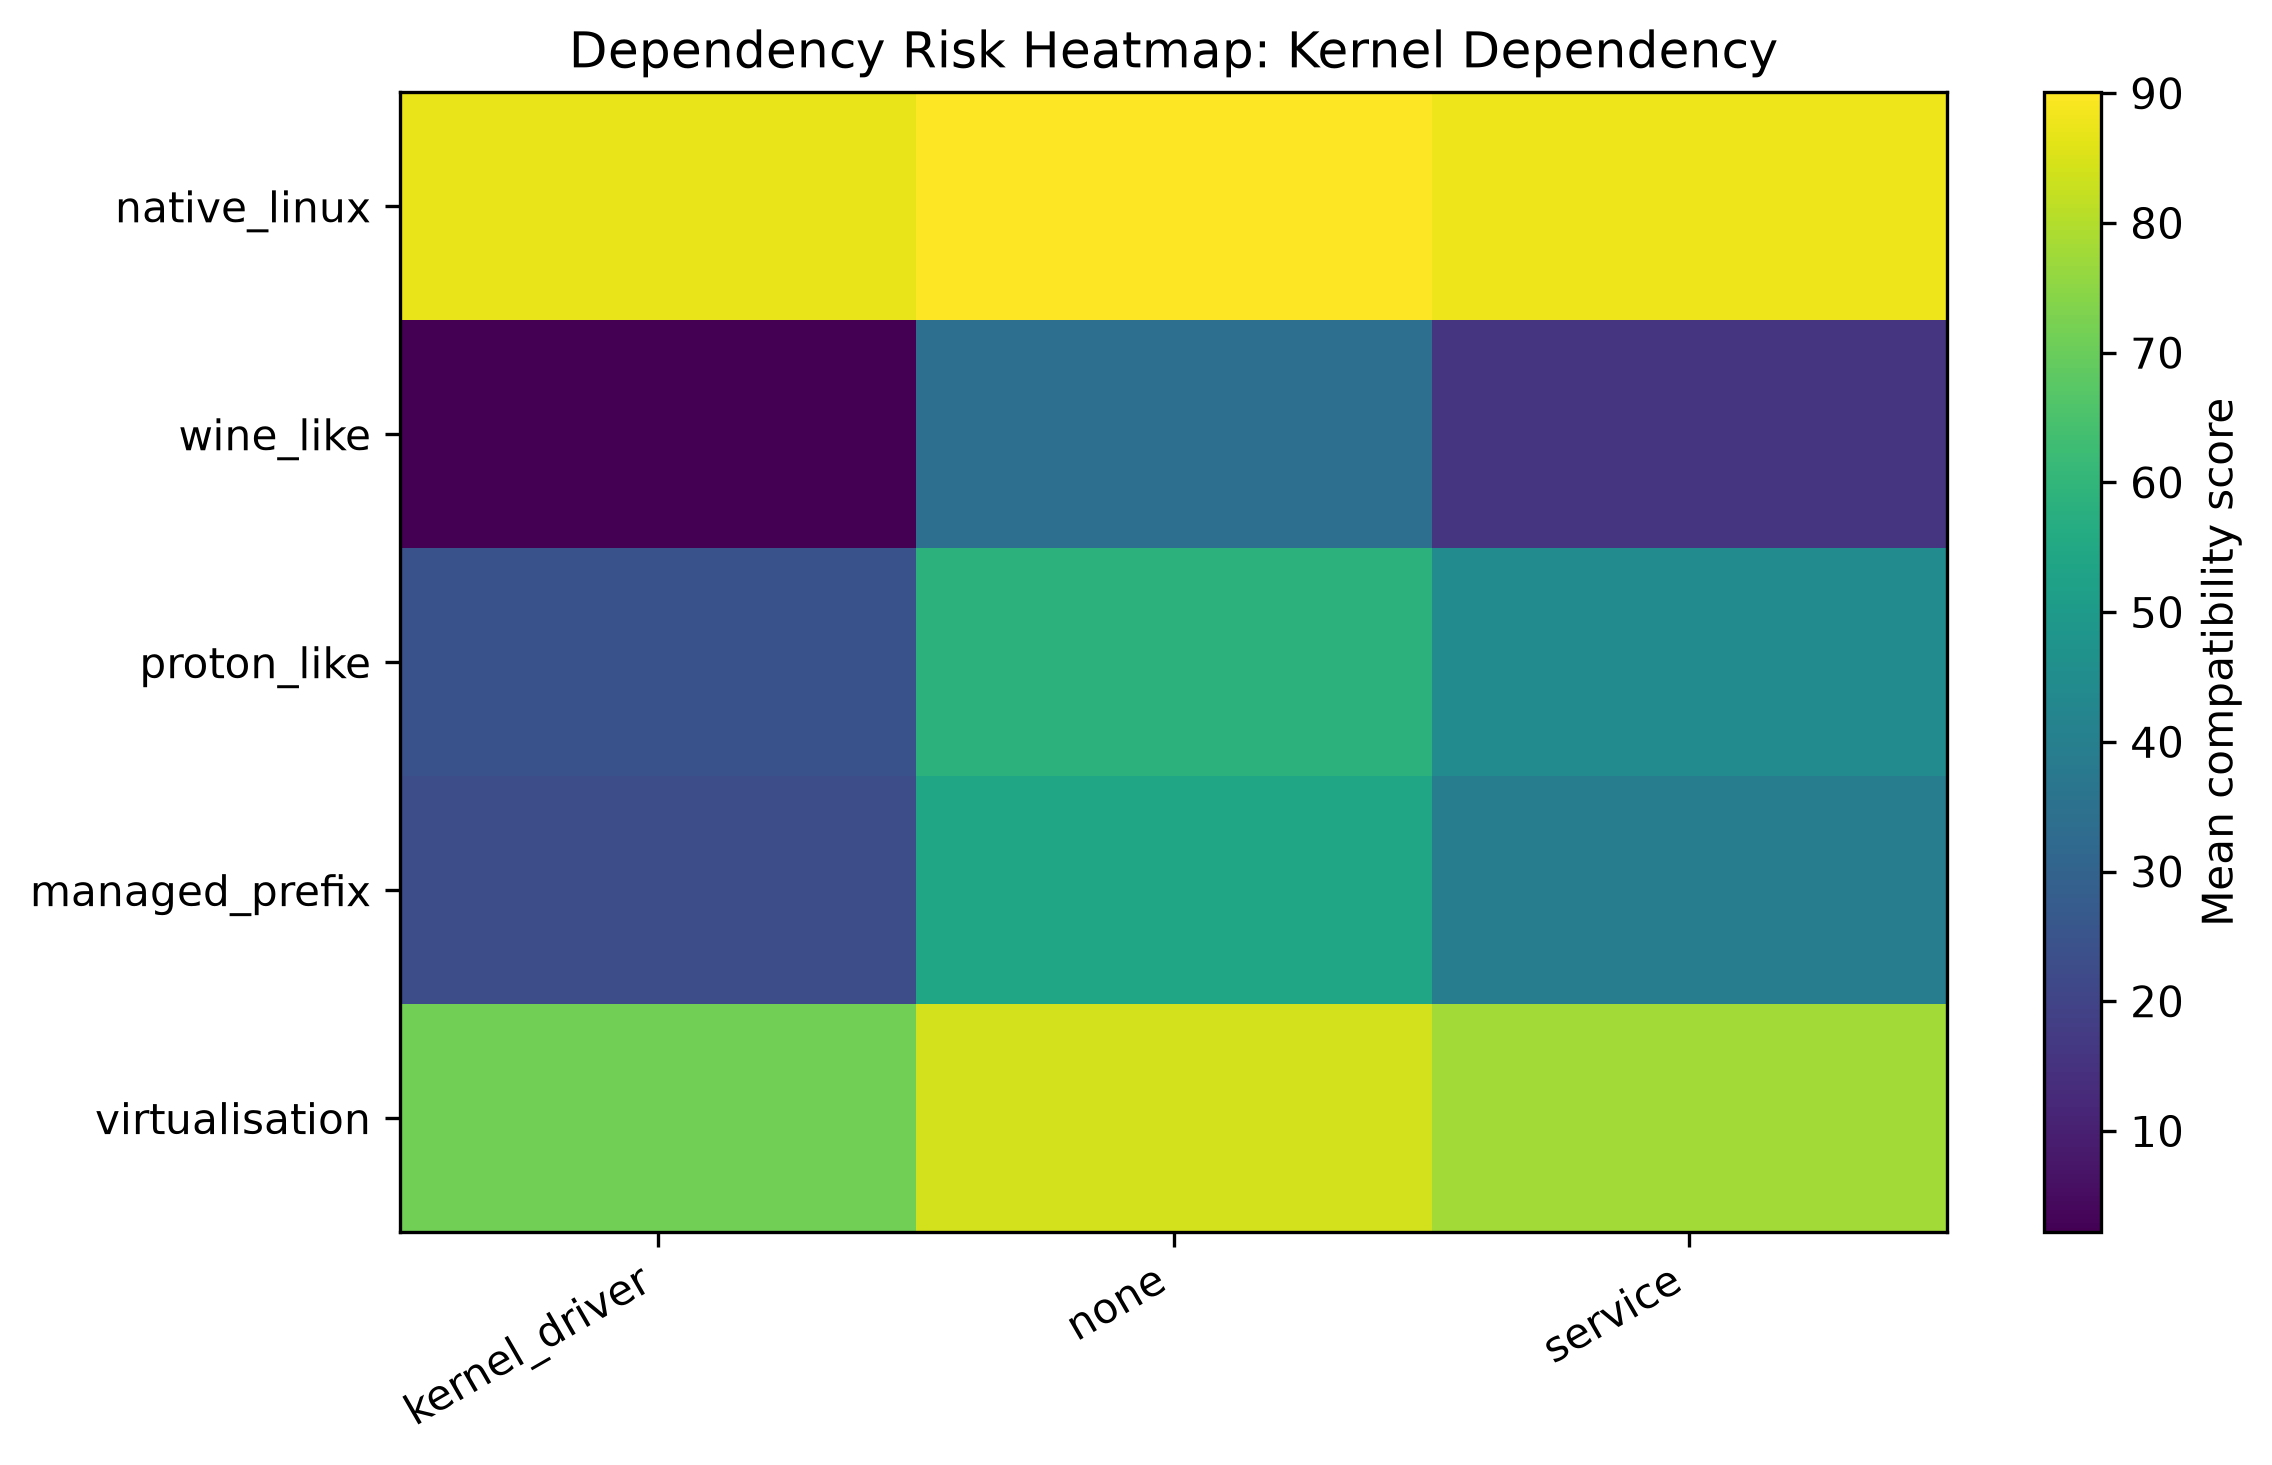
\includegraphics[width=\linewidth]{dependency_risk_heatmap.png}
    \caption{Synthetic dependency-risk heatmap.}
    \label{fig:dependency-risk}
\end{figure}

\begin{figure}[t]
    \centering
    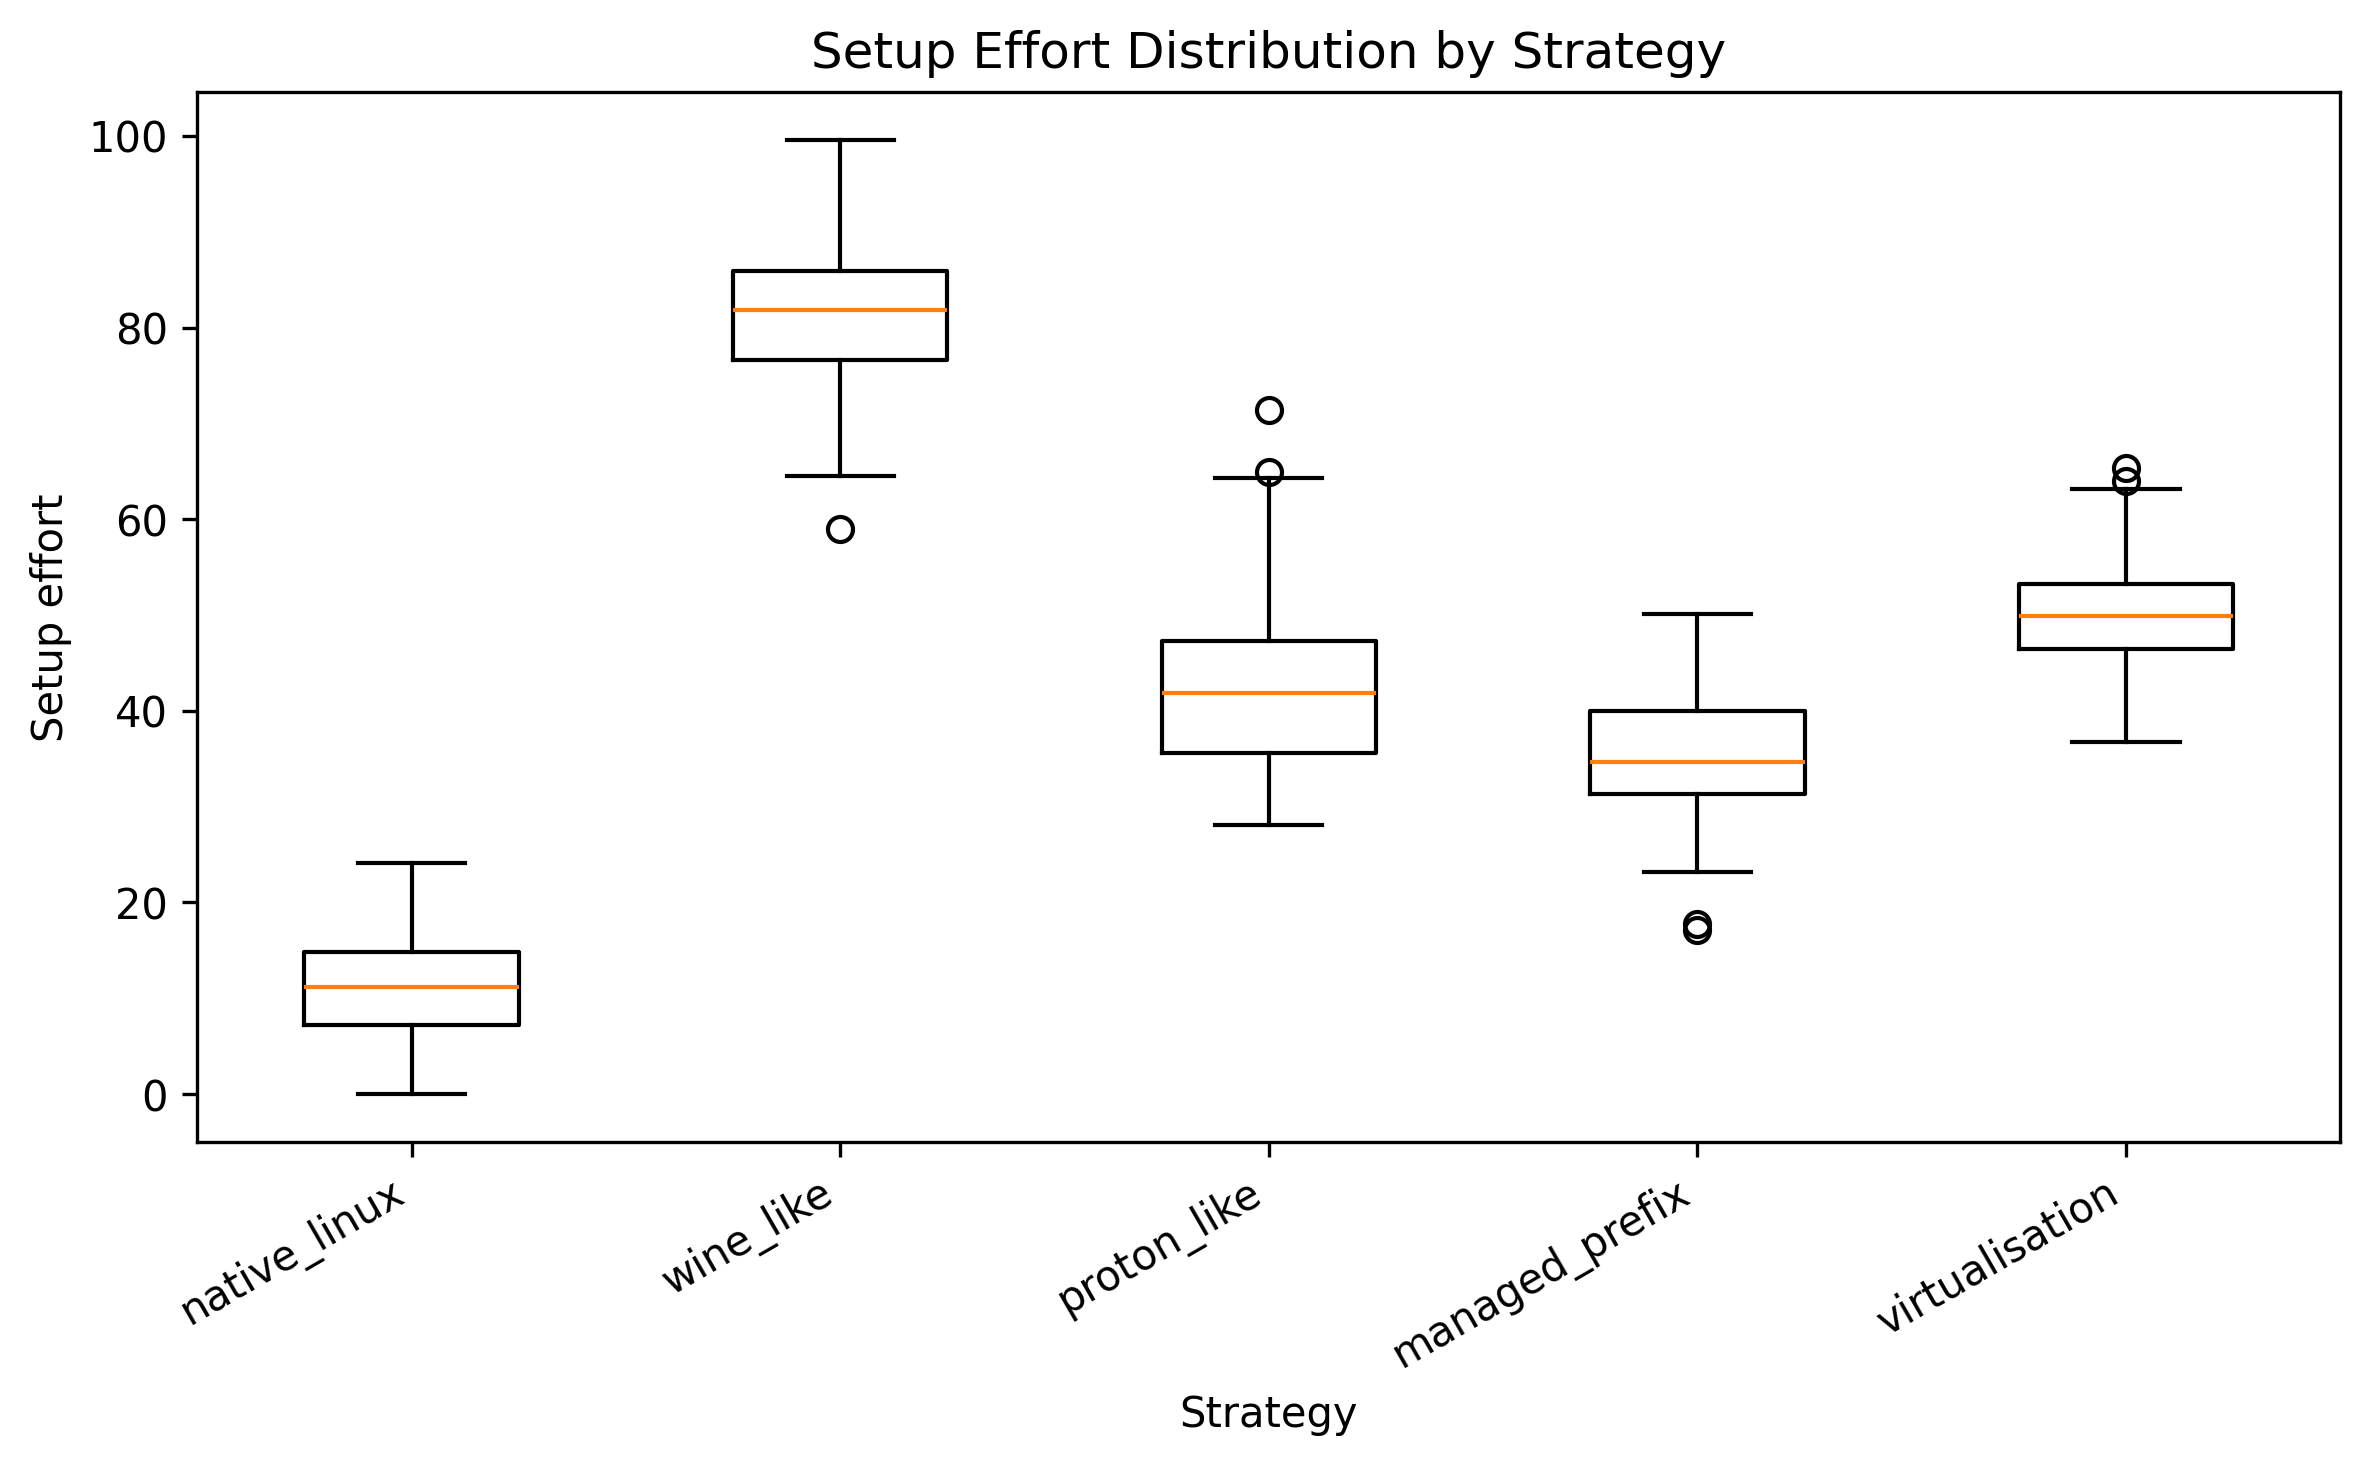
\includegraphics[width=\linewidth]{setup_effort_boxplot.png}
    \caption{Synthetic setup effort distribution by strategy.}
    \label{fig:setup-effort}
\end{figure}

\section{Discussion}

\subsection{Compatibility Layers Reduce but Do Not Erase the Barrier}

The analysis suggests that compatibility layers can reduce the Windows--Linux application barrier for some workloads. This is especially plausible for applications whose main dependencies are user-space APIs or graphics calls that can be translated.

However, compatibility layers are weaker when the dependency is outside user-space API translation. Kernel drivers, anti-cheat systems, licensing services, proprietary hardware and enterprise workflows remain difficult.

\subsection{Proton as Evidence of Engineering Feasibility}

Proton demonstrates that compatibility-layer engineering can support complex workloads when it is combined with platform integration. Its significance lies in the combination of Wine-based compatibility, graphics translation, runtime control and Steam integration.

The key lesson is not that every Windows application can run on Linux. The key lesson is that compatibility can become practical when the compatibility layer is embedded in a broader technical and distribution ecosystem.

\subsection{Bazzite as Distribution-Level Evidence}

Bazzite adds a different kind of evidence. It does not directly reimplement Windows APIs. Instead, it reduces friction around using a Linux system for gaming and compatibility workflows.

This supports a broader conclusion: compatibility-layer success depends not only on API coverage, but also on the operating-system environment surrounding the compatibility layer.

\subsection{Virtualisation as Fallback}

Virtualisation remains important because it can support applications that compatibility layers cannot. However, it preserves Windows as a required component. It therefore reduces short-term migration friction but does not remove Windows dependence.

\subsection{Implications for Linux Adoption}

The Windows--Linux adoption problem should be understood as a layered issue: application binary compatibility, runtime and dependency management, graphics and driver support, licensing and service compatibility, distribution-level usability and organisational workflow migration. Solving only one layer is not enough.

\section{Limitations}

This paper has several limitations.

First, the experiment is synthetic. It does not measure real applications and should not be presented as a benchmark.

Second, the model uses manually defined weights. These weights are transparent and reproducible, but they are still assumptions.

Third, Proton evidence is gaming-oriented. The paper uses gaming as a demanding case study, but it must avoid generalising directly from games to all Windows software.

Fourth, community compatibility databases such as ProtonDB can provide useful practical context, but they are not controlled scientific evidence \cite{protondb}.

Fifth, compatibility changes over time. Wine, Proton, SteamOS, Bazzite, drivers, applications and DRM systems are all moving targets.

Sixth, the paper does not perform a legal or economic analysis of licensing, vendor lock-in or digital sovereignty. These topics are used only to frame motivation.

\section{Conclusion}

The Windows--Linux application barrier remains one of the main obstacles to desktop Linux adoption. It is not caused by a single technical limitation of Linux, but by the accumulated dependency of applications, workflows and organisations on Windows-specific APIs, services, drivers, licensing mechanisms and platform assumptions.

The state of the art suggests, however, that this barrier is no longer immovable. Wine provides the general compatibility-layer foundation, while Proton and SteamOS show that complex Windows workloads can become practical on Linux when API translation, graphics translation, runtime control and platform integration are engineered together. Bazzite further illustrates that distribution-level engineering can reduce adoption friction by making the surrounding Linux environment more coherent, preconfigured and resilient.

The most important result is therefore not that compatibility layers already solve every case, but that they substantially change the feasibility of migration. Kernel drivers, anti-cheat systems, proprietary licensing, specialised hardware, cloud services and enterprise workflows remain difficult barriers. Yet these limitations define the remaining frontier rather than proving that the Windows compatibility barrier is permanent.

For this reason, the future of Windows--Linux portability should be understood as an engineering and ecosystem challenge rather than as a fixed structural impossibility. If compatibility layers, native ports, open standards and distribution-level integration continue to improve, Linux could become a more realistic desktop alternative for users and organisations currently constrained by Windows-only software. Breaking the compatibility barrier would therefore have consequences beyond technical convenience: it would reduce vendor lock-in, strengthen user choice and support a computing ecosystem less dependent on a single dominant proprietary platform.

\bibliographystyle{IEEEtran}
\bibliography{references}

\end{document}
